\documentclass[12pt,letterpaper,oneside]{book} 
%\documentclass[12pt,twoside,letterpaper]{book}
% oneside indica que nao � frente e verso

% ---------------------------------------------------------------------------- %
% Pacotes 
\usepackage[T1]{fontenc}
\usepackage[brazil]{babel}
%\usepackage[latin1]{inputenc}
\usepackage[pdftex]{graphicx}           % usamos arquivos pdf/png como figuras
\usepackage{setspace}                   % espa�amento flex�vel
\usepackage{indentfirst}                % indenta��o do primeiro par�grafo
\usepackage{makeidx}                    % �ndice remissivo
\usepackage[nottoc]{tocbibind}          % acrescentamos a bibliografia/indice/conteudo no Table of Contents
\usepackage{courier}                    % usa o Adobe Courier no lugar de Computer Modern Typewriter
\usepackage{type1cm}                    % fontes realmente escal�veis
\usepackage{listings}                   % para formatar c�digo-fonte (ex. em Java)

\usepackage{titletoc}
\usepackage{booktabs}                   % para gera��o de tabelas
\usepackage[bf,small,compact]{titlesec} % cabe�alhos dos t�tulos: menores e compactos
\usepackage[fixlanguage]{babelbib}
\usepackage[font=small,format=plain,labelfont=bf,up,textfont=it,up]{caption}
\usepackage[usenames,svgnames,dvipsnames]{xcolor}
\usepackage[a4paper,top=2.54cm,bottom=2.0cm,left=2.0cm,right=2.54cm]{geometry} % margens
\usepackage[pdftex,plainpages=false,pdfpagelabels,pagebackref,colorlinks=true,citecolor=black,linkcolor=black,urlcolor=black,filecolor=black,bookmarksopen=true]{hyperref} % links em preto
% \usepackage[pdftex,plainpages=false,pdfpagelabels,pagebackref,colorlinks=true,citecolor=DarkGreen,linkcolor=NavyBlue,urlcolor=DarkRed,filecolor=green,bookmarksopen=true]{hyperref} % links coloridos
\usepackage[all]{hypcap}                    % soluciona o problema com o hyperref e capitulos
%\usepackage[square,sort,nonamebreak,comma]{natbib}  % cita��o bibliogr�fica alpha (alpha-ime.bst)

% By David
\usepackage{amsthm}
\usepackage{acronym} 
% \usepackage[portugues,ruled,vlined,linesnumbered]{algorithm2e/algorithm2e}
\usepackage{supertabular}

% By Suelen
\usepackage{gensymb}
\usepackage[bottom]{footmisc}

% ---------------------------------------------------------------------------- %
% Cabe�alhos similares ao TAOCP de Donald E. Knuth
\usepackage{fancyhdr}
\pagestyle{fancy}
\fancyhf{}
\renewcommand{\lstlistingname}{C�digo-fonte}
\renewcommand{\chaptermark}[1]{\markboth{\MakeUppercase{#1}}{}}
\renewcommand{\sectionmark}[1]{\markright{\MakeUppercase{#1}}{}}
\renewcommand{\headrulewidth}{0pt}

% ---------------------------------------------------------------------------- %
\graphicspath{{./figuras/}}             % caminho das figuras (recomend�vel)
\frenchspacing                          % arruma o espa�o: id est (i.e.) e exempli gratia (e.g.) 
\urlstyle{same}                         % URL com o mesmo estilo do texto e n�o mono-spaced
\makeindex                              % para o �ndice remissivo
\raggedbottom                           % para n�o permitir espa�os extra no texto
\fontsize{60}{62}\usefont{OT1}{cmr}{m}{n}{\selectfont}
\cleardoublepage
\normalsize

% ---------------------------------------------------------------------------- %
% Op��es de listing usados para o c�digo fonte
% Ref: http://en.wikibooks.org/wiki/LaTeX/Packages/Listings
\lstset{ %
language=Java,                  % choose the language of the code
basicstyle=\footnotesize,       % the size of the fonts that are used for the code
numbers=left,                   % where to put the line-numbers
numberstyle=\footnotesize,      % the size of the fonts that are used for the line-numbers
stepnumber=1,                   % the step between two line-numbers. If it's 1 each line will be numbered
numbersep=5pt,                  % how far the line-numbers are from the code
showspaces=false,               % show spaces adding particular underscores
showstringspaces=false,         % underline spaces within strings
showtabs=false,                 % show tabs within strings adding particular underscores
frame=single,	                % adds a frame around the code
framerule=0.6pt,
tabsize=2,	                    % sets default tabsize to 2 spaces
captionpos=b,                   % sets the caption-position to bottom
breaklines=true,                % sets automatic line breaking
breakatwhitespace=false,        % sets if automatic breaks should only happen at whitespace
escapeinside={\%*}{*)},         % if you want to add a comment within your code
backgroundcolor=\color[rgb]{1.0,1.0,1.0}, % choose the background color.
rulecolor=\color[rgb]{0.8,0.8,0.8},
extendedchars=true,
xleftmargin=\parindent,
xrightmargin=\parindent,
framexleftmargin=15pt,
framexrightmargin=15pt
}


\pagestyle{headings}
\markboth{}{}

% ---------------------------------------------------------------------------- %
% Dimens�es da p�gina (letterpaper)
%\setlength{\paperwidth}{216mm}
%\setlength{\topmargin}{1.3cm}         % deslocamento do topo do texto 
%\setlength\oddsidemargin{0cm}
%\setlength\evensidemargin{0cm}
%\setlength{\parskip}{1.2mm}
%\setlength{\parindent}{4mm}
%\setlength{\textwidth}{135mm}          % largura do texto
%\setlength{\parindent}{0pt}
%\setlength{\textheight}{22cm}
%\setlength{\parskip}{0.2cm}


\newcommand{\eb}{\varepsilon}
\newcommand{\mdp}{\langle\mathcal{S,A},p,r,c\rangle}
\newcommand{\ctlstar}{{\sc ctl}$^\star$}
\newcommand{\ctl}{\sc ctl}
\newcommand{\ltl}{\sc ltl}
\newtheorem{Def}{Defini��o}[chapter]
\newtheorem{Teo}{Teorema}[chapter]
\newtheorem{Ex}{Exemplo}[section]
\newtheorem{Tab}{Tabela}[chapter]

\begin{document}
%\hypersetup{
%pdfauthor = {Suelen Goularte Carvalho},
%pdftitle = {Algo Relacionado a Mobile},
%pdfsubject = {Disserta��o de Mestrado},
%pdfkeywords={Mobile, Computa��o Movel, Celular} % <== Precisa rever o que vai colocar aqui !!!
%pdfcreator = {LaTeX with hyperref package},
%}

\frontmatter

\onehalfspacing
% -*- root: dissertacao.tex -*-
\thispagestyle{empty}
\begin{center}
    \vspace*{2cm}
    \large{\textbf{Detec��o de Anomalias na Camada de Apresenta��o\\
    de Aplicativos Android Nativos}}\\
	
    \vspace*{1.2cm}
    Suelen Goularte Carvalho \\ 
    
    \vskip 2cm
	\textsc{
	Disserta��o apresentada\\[-0.25cm] 
	ao\\[-0.25cm]
	Instituto de Matem�tica e Estat�stica\\[-0.25cm]
	da\\[-0.25cm]
	Universidade de S�o Paulo\\[-0.25cm]
	para\\[-0.25cm]
	obten��o do t�tulo\\[-0.25cm]
	de\\[-0.25cm]
	Mestre em Ci�ncias}
    
    \vskip 1.5cm
    Programa: Mestrado em Ci�ncia da Computa��o\\
    Orientador: Marco Aur�lio Gerosa, Ph.D.\\
   
    % \vskip 1.5cm

    \vskip 1cm
	\normalsize{}
	
    \vskip 0.5cm
    \normalsize{S�o Paulo, Julho de 2016}

\end{center}

% P�gina de rosto
\newpage
\thispagestyle{empty}
	\begin{center}
    	\vspace*{0.2 cm}
        \large{\textbf{Detec��o de Anomalias na Camada de Apresenta��o\\
    	de Aplicativos Android Nativos}}\\
	    \vspace*{2 cm}
	\end{center}

	\vskip 2cm

	\begin{flushright}
	Esta � a vers�o original da disserta��o elaborada\\
	pela candidata Suelen Goularte Carvalho, tal como\\
	submetida a Comiss�o Julgadora.\\
	\vskip 3cm

	\end{flushright}
	\vskip 4.2cm

	\begin{quote}
	\noindent Comiss�o Julgadora:
	
	\begin{itemize}
		\item {Marco Aur�lio Gerosa, Ph.d. $-$ IME-USP}
		\item {Alfredo Goldman vel Lejbman, Ph.d. $-$ IME-USP}
		\item {Paulo Roberto Miranda Meirelles, Ph.d. $-$ IME-USP}
	\end{itemize}
	  
	\end{quote}

\newpage
\thispagestyle{empty}
	\vspace*{12cm}
	\vskip 1cm

	\begin{flushright}
	{\small Dedico esta disserta��o de mestrado a minha m�e.\\}
	\end{flushright}

	\vspace*{1cm}

	\begin{flushright}
	{\it ``O motivo do tempo � que tudo n�o acontece de uma vez s�.''} \\
	$-$ Albert Einstein
	\end{flushright}

\pagebreak


\pagenumbering{roman}

\onehalfspacing
% \chapter*{Agradecimentos}
\setlength{\parindent}{0mm}

A fazer. \\

% -*- root: dissertation.tex -*-
\noindent CARVALHO, G. S. \textbf{Bad smells on the Android front-end: A study on the developers' perception}. 
2018. %100 f.
Disserta��o (Mestrado) - Instituto de Matem�tica e Estat�stica,
Universidade de S�o Paulo, S�o Paulo, 2018.
\\

There is no question that good codes matter, but how do you know when a code is not good? Bad smells of code help us identify problematic code snippets, but most of the bad odors cataloged are based on traditional technologies, created from the 1970s through the 90s, such as Java. There are still doubts about bad smells in technologies that have emerged in the last decade, such as Android, the main mobile platform in 2017 with more than 86\% market share. Some researchers have defined new bad smells related to Android eficience and usability. Other research concludes that the components most affected by traditional bad smells are related to the front-end, such as \textit{Activities} and \textit{Adapters}. Also noticed in some applications, front-end codes represent a larger part. It is noteworthy that the Android front-end is also composed of XML files, called application resources, used for a user interface (UI) construction, but these files were not considered in their analyzes. In this dissertation, we investigate existence of bad smells of code related to the Android front-end considering even application resources. We did this through 2 online surveys and 3 experiments summing 3XX developers. Our results showed that there is a common perception among practicing Android developers about bad practices no Android front-end. Our main contributions are a set of 13 bad smells from the Android front-end and a statistical analysis of the perceptions of practitioner developers about the bad smells set. Our contributions will serve researchers as a starting point for the definition of heuristics and implementation of automated tools and to practitioner developers as an aid in identifying problematic codes to be improved, even manually.


\noindent \textbf{Palavras-chave:} Android, bad smells, software quality, software maintance.

\onehalfspacing
\tableofcontents

\chapter{Lista de Abreviaturas}

\begin{acronym}

\acro{SDK}{{\it Software Development Kit}} % 
\acro{IDE}{{\it Integrated Development Environment}} % 
\acro{APK}{{\it Android Package}} % 
\acro{ART}{{\it Android RunTime}} % 

\end{acronym}


% \chapter{Lista de S�mbolos}

\begin{supertabular}{ll}


$\Sigma$ & Sistema de transi��o de estados \\


\end{supertabular}


\listoffigures
% \listofalgorithms

\mainmatter

%%%%%%%%%%%%%%%%%%%%%%%%%%%%%%%%%%%%%%%%%%%%%%%%%%%%%%%%%%%%%%%%%%%%%%%%%
\onehalfspacing

% -*- root: dissertation.tex -*-
% \lettrine[nindent=0em,lines=3]{L}orem ipsim ult as 
Escrever c�digo com qualidade tem se tornado cada vez mais importante com o aumento da complexidade de tecnologias e anseio dos usu�rios por novas funcionalidade e atualiza��es \cite{Hecht2015,MobileSmells:13}. Existem diferentes pr�ticas, padr�es e ferramentas que auxiliam os desenvolvedores a escrever c�digo com qualidade, incluindo \textit{design patterns} \cite{gof} e cheiros de c�digo \cite{Refactoring:99}. A falta de qualidade resulta em defeitos de software que custam a empresas quantias significativas, especialmente quando conduzem a falhas de software \cite{Nagappan:2005, briand1993modeling}. Evolu��o e manuten��o de software tamb�m j� se provaram como os maiores gastos com aplica��es \cite{RefactoringAndImprovements:10}.

Uma das formas de aumentar a qualidade de software � identificar trechos de c�digos ruins e refator�-los, ou seja, alterar o c�digo sem alterar o comportamento \cite{Refactoring:99}. Desta forma, temos que cheiros de c�digo s�o aliados importantes na busca por qualidade de c�digo pois, representam sintomas que podem indicar problemas mais profundos no software, n�o necessariamente, sendo o problema em si \cite{CodeSmell:06}. Seu mapeamento possibilita a defini��o de heur�sticas que, por sua vez, possibilitam a implementa��o de ferramentas que os identificam de modo autom�tico no c�digo. PMD \cite{PMD2016}, Checkstyle e FindBugs s�o exemplos de ferramentas que identificam automaticamente alguns tipos de cheiros de c�digo em projetos Java. 

Enquanto que cheiros de c�digo em projetos Java j� foram extensivamente estudados \cite{Riel, Refactoring:99, Martin:2008:CCH:1388398}, ainda h� muito a se pesquisar sobre cheiros de c�digo em projetos Android. No entanto, determinar o que � ou n�o um cheiro de c�digo � subjetivo e pode variar de acordo com a tecnologia, desenvolvedor, metodologia de desenvolvimento dentre outros aspectos \cite{WikiCodeSmell}. Em particular, Aniche et al. \cite{MvcSmells:16,aniche2016satt} mostraram que a arquitetura do software � um fator importante e que deve ser levada em conta ao analisar a qualidade de um sistema. Outros estudos identificaram cheiros de c�digo espec�ficos Android relacionados ao consumo inteligente de recursos do dispositivo, como bateria e mem�ria, usabilidade, dentre outros \cite{EnergyAndroidSmells, ReimannBrylski2013}. Verloop \cite{MobileSmells:13} analisou se classes derivadas do SDK Android s�o mais ou menos propensas a cheiros de c�digo tradicionais do que classes puramente Java. Linares et al. \cite{DomainMatters} usaram o m�todo DECOR para realizar a detec��o de 18 \textit{anti-patterns} orientado a objetos em aplicativos m�veis.

% Umme et al. \cite{Mannan_Dig_Ahmed_Jensen_Abdullah_Almurshed} recentemente levantaram que, das principais confer�ncias de manuten��o de software (ICSE, FSE, OOPSLA/SPLASH, ASE, ICSM/ICSME, MRS e ESEM), dentre 2008 a 2015, apenas 10\% dos artigos consideraram em suas pesquisas, projetos Android. Nenhuma outra plataforma m�vel foi considerada.  

Nossa pesquisa complementa as anteriores no sentido de que tamb�m buscamos por cheiros de c�digo Android. E se difere delas pois buscamos cheiros de c�digo relacionados � qualidade, em termos de manutenabilidade e legibilidade, espec�fico dessa plataforma. Por exemplo \textsc{Activities}, \textsc{Fragments} e \textsc{Adapters} s�o classes usadas na constru��o de telas e \textsc{listeners} s�o respons�veis pelas intera��es com os usu�rios. Buscamos entender ent�o quais s�o as \emph{boas e m�s} pr�ticas no desenvolvimento da interface visual Android. 

% Para limitar nosso objeto de estudo, optamos por focar em cheiros de c�digo relacionados ao \textit{front-end} Android pois encontramos pesquisas com abordagem similar, por�m relacionadas ao \textit{front-end} de tecnologias web, como CSS \cite{CSSCodeSmell}, Javascript \cite{BB} e o arcabou�o Spring MVC \cite{FinavaroAniche2016}. 

% E enquanto que cheiros de c�digo em projetos Java j� foram extensivamente estudados \cite{Riel, Refactoring:99, Martin:2008:CCH:1388398}, o \textit{front-end} Android ainda carece de estudo e possui peculiaridades n�o encontradas em c�digo Java tradicional \cite{Mannan_Dig_Ahmed_Jensen_Abdullah_Almurshed}. Alguns exemplos dessas peculiaridas s�o o ciclo de vida de \textsc{Activities} e \textsc{Fragments} e a cria��o da interface visual que � feita atrav�s de arquivos XML chamados de \textsc{layout resources}.
 

Por meio de um question�rio online com perguntas sobre boas e m�s pr�ticas relacionadas ao \textit{front-end} Android respondido por 45 desenvolvedores, derivamos 23 m�s pr�ticas. Validamos a percep��o dos desenvolvedores sobre essas m�s pr�ticas atrav�s de um experimento com outros 20 desenvolvedores. Os resultados mostram que de fato existem boas e m�s pr�ticas espec�ficas ao \textit{front-end} Android. Ainda que tenhamos validado com sucesso a percep��o dos desenvolvedores sobre apenas duas, esperamos que este cat�logo de m�s pr�ticas possa contribuir com ideias iniciais para outras pesquisas sobre qualidade de codigo em projetos Android.

 % para a defini��o de cheiros de c�digo e heur�sticas para a detec��o sistematizada das mesmas em projetos Android, al�m de contribuir com sugest�es de como mitig�-las.

As contribui��es deste trabalho s�o:

\begin{enumerate}

	\item Cat�logo com 23 m�s pr�ticas e sugest�es de solu��es no desenvolvimento do \textit{front-end} Android, derivadas a partir dos resultados obtidos com a aplica��o de um question�rio online respondido por 45 desenvolvedores.

	\item A percep��o de desenvolvedores sobre as quatro m�s pr�ticas de alta recorr�ncia atrav�s de um experimento online com 20 desenvolvedores. Obtivemos um resultado positivo e estat�sticamente v�lido sobre duas delas.

	\item Ap�ndice online~\cite{apendice} com roteiros dos question�rios e outras informa��es da pesquisa para que outros pesquisadores possam replicar nosso estudo.

\end{enumerate}


% \begin{enumerate}
% 	\item Cat�logo com 23 m�s pr�ticas no desenvolvimento do \textit{front-end} Android, derivadas a partir dos resultados obtidos com a aplica��o de um question�rio online respondido por 45 desenvolvedores.
% 	\item A percep��o de desenvolvedores sobre as quatro m�s pr�ticas mais recorrentes atrav�s de um question�rio online com 11 desenvolvedores..
% 	\item Ap�ndice online \footnote{Ap�ndice online: http://suelengc.com/android-code-smells-article} com roteiros dos quetion�rios e outras informa��es da pesquisa para que outros pesquisadores possam replicar nosso estudo.
% \end{enumerate}

As se��es seguintes deste artigo est�o organizadas da seguinte forma: a Se��o \ref{metodologia} aborda a metodologia de pesquisa. A Se��o \ref{resultados} apresenta o cat�logo de m�s pr�ticas a percep��o de desenvovledores sobre as quatro mais recorr�ntes. A Se��o \ref{ameacas} aborda as amea�as � validade do estudo. A Se��o \ref{relacionados} discute os trabalhos relacionados e o estado da arte sobre Android e cheiros de c�digo. E por fim, a Se��o \ref{conclusao} conclui.
 
% -*- root: dissertacao.tex -*-
%%%%%%%%%%%%%%%%%%%%%%%%%%%%%%%%%%%%%%%%%%%%%%%%%%%%%%%%%%%%%%%%%%%%%%%
\setlength{\parindent}{20pt}
\setlength{\textheight}{22cm}
\setlength{\parskip}{0.2cm}
\linespread{1.2} % Para aumentar o espa�amento entre as linhas
%%%%%%%%%%%%%%%%%%%%%%%%%%%%%%%%%%%%%%%%%%%%%%%%%%%%%%%%%%%%%%%%%%%%%%%

\chapter{Fundamenta��o Conceitual}
\label{cap:background}

Para a compreens�o deste trabalho � importante ter compreens�o de dois temas: Maus Cheiros de C�digo e Android.

% \section{Refatora��o}


\section{Maus Cheiros de C�digo}
\label{sec:MausCheiros}

Maus cheiros de c�digo s�o sintomas de design ruim e m�s pr�ticas de programa��o \cite{WikiCodeSmell, FinavaroAniche2016, Refactoring:99, MobileSmells:13}. Tamb�m conhecido por anomalias de c�digo \cite{padilha2013detecccao}. Diferentemente de erros sist�micos, eles n�o resultam em comportamentos err�neos \cite{WikiCodeSmell, MobileSmells:13}. Maus cheiros apontam fraquezas no \textit{design} que podem desacelerar o desenvolvimento e aumentar o risco a defeitos, falhas e mudan�as \cite{WikiCodeSmell, FinavaroAniche2016, Khomh:2012:ESI:2158916.2158921, DomainMatters}. Do ponto de vista do desenvolvedor, maus cheiros s�o heur�sticas para refatora��es que indicam quando refatorar e qual t�cnica de refatora��o usar \cite{WikiCodeSmell}.

Refatora��o � definido por Fowler como ``uma t�cnica para reestrutura��o de um c�digo existente, alterando sua estrutura interna sem alterar seu comportamento externo'' \cite{Refactoring:99}. Escolher n�o resolver um mau cheiro pela refatora��o n�o resultar� na aplica��o falhar mas ir� aumentar a dificuldade de mant�-la. A refatora��o ajuda a melhorar a manutenibilidade de uma aplica��o \cite{MobileSmells:13}. Uma vez que os custos com manuten��o s�o a maior parte dos custos envolvidos no ciclo de desenvolvimento de software, aumentar a manutenibilidade atrav�s de refatora��o ir� reduzir os custos de um software no longo prazo \cite{RefactoringAndImprovements:10}. 

O livro de Webster (1995) \cite{Webster} deve ter sido um dos primeiros onde o termo cheiro de c�digo, referindo-se a m�s pr�ticas, foi usado. Mais adiante, \textbf{mau cheiro de c�digo} foi usado por Martin Fowler e Kent Beck no livro Refactoring (1999) \cite{Refactoring:99} referindo-se a um trecho de c�digo que pode se beneficiar de refatora��o. Em uma postagem em 2006 em seu site \cite{CodeSmell:06}, Martin Fowler define um \textbf{cheiro de c�digo} como sendo ``uma indica��o superficial no c�digo que usualmente corresponde a um problema mais profundo no sistema'' e complementa dizendo que ``primeiramente um mau cheiro � por defini��o algo r�pido de ser detectado - farej�vel - e segundo, que um mau cheiro nem sempre indica um problema' (tradu��o livre). 

Note que o termo usado no livro Refactoring (1999) \cite{Refactoring:99} � mau cheiro de c�digo (\textit{bad smell in code}) e na postagem em seu site \cite{CodeSmell:06} � cheiro de c�digo (\textit{code smell}). Essa diferen�a pode ser justificada pela afirmativa de Fowler, na postagem em seu site, em que diz que ``cheiros de c�digo n�o s�o inerentemente ruins por conta pr�pria - eles s�o muitas vezes um indicador de um problema e n�o o problema em si'' (tradu��o livre).

No livro Refactoring for Software Design Smells (2014) \cite{Suryanarayana2014Refactoring} encontramos uma defini��o sobre cheiro de c�digo relacionada a princ�pios e qualidade, onde diz que ``[cheiros de c�digo] s�o certas estruturas que indicam viola��o de princ�pios de \textit{design} fundamentais e impactam negativamente na qualidade do \textit{design}''. De fato, pesquisas t�m apontado que maus cheiros de c�digo est�o relacionados � degrada��o da qualidade em projetos de software \cite{ReimannBrylski2013}.

Outro termo comum de se ver juntamente com (mau) cheiro de c�digo � o termo \textit{antipattern}, tamb�m conhecido como m� pr�tica. Esse, por sua vez, descreve uma solu��o comum para um problema que gera consequ�ncias negativas \cite{WilleyAntiPatterns}. Pode ser resultado de um desenvolvedor n�o ter conhecimento suficiente ou experi�ncia em resolver um determinado tipo de problema, ou ter aplicado um \textit{design pattern}, solu��o reutiliz�vel para um problema de \textit{design} recorrente \cite{WilleyAntiPatterns, gof}, perfeitamente bom no contexto errado \cite{WilleyAntiPatterns}. Geralmente, (maus) cheiros de c�digo s�o sintomas da presen�a de \textit{antipattern}. Linares et al. \cite{DomainMatters} concluem que \textit{antipatterns} impactam de forma negativa aplica��es m�veis, em particular m�tricas de qualidade relacionadas ao aumento do risco de falhas.

Para auxiliar no processo de refatora��o, � comum desenvolvedores se utilizarem de ferramentas de detec��o de cheiros de c�digo \cite{FinavaroAniche2016}, sintomas de design ruim e m�s pr�ticas de programa��o \cite{WikiCodeSmell, FinavaroAniche2016, Refactoring:99, MobileSmells:13}. Para automatizar a detec��o de cheiros de c�digo, � importante t�-los mapeados e catalogados. Muitos cheiros de c�digo j� foram catalogados \cite{Refactoring:99,Suryanarayana2014Refactoring, Webster}. 

Diversos autores j� trabalharam na defini��o de diferentes cat�logos de cheiros de c�digo. Riel \cite{Riel} definiu mais de 60 caracter�sticas de um bom c�digo orientado a objetos. Fowler \cite{Refactoring:99} definiu mais de 20 maus cheiros como \textit{God Classes} \cite{Refactoring:99}, que s�o classes que fazem ou sabem muitas coisas e \textit{Feature Envy} \cite{Refactoring:99}, que s�o m�todos que est�o mais interessados em outras classes do que na pr�pria classe. Existem diversas ferramentas atualmente que conseguem realizar a detec��o autom�tica de diversos desses maus cheiros como PMD \cite{PMD2016} e Sonar \cite{Sonarqube2016}.

No entanto, nas principais confer�ncias de manuten��o de software, dentre 2008 a 2015, 5 de um total de 52 artigos, foram sobre maus cheiros Android \cite{Mannan_Dig_Ahmed_Jensen_Abdullah_Almurshed}. A aus�ncia de um cat�logo de maus cheiros Android resulta em (i) uma car�ncia de conhecimento sobre boas e m�s pr�ticas a ser compartilhado entre praticantes da plataforma, (ii) indisponibilidade de uma ferramenta de detec��o de maus cheiros de modo a alertar automaticamente os desenvolvedores de sua exist�ncia e (iii) aus�ncia de estudo emp�rico sobre o impacto dessas m�s pr�ticas na manutenibilidade do c�digo de projetos Android. 

Nesta disserta��o utilizamos o termo \textbf{cheiro de c�digo} para nos referir a ambos os termos (mau) cheiro de c�digo, \textit{antipattern} e anomalias de c�digo, como em trabalhos pr�vios \cite{DomainMatters, Moha_Gueheneuc_Meur_Duchien_2008, padilha2013detecccao}, e nosso foco est� em definir e detectar maus cheiros relacionados especificamente � camada de apresenta��o de projetos Android.

\section{Android}
\label{sec:Android}

Atualmente o Android � a plataforma m�vel com maior crescimento. Em 2017 completar� uma d�cada do seu lan�amento \cite{AndroidHistory}. A Figura \ref{fig:AndroidMarketShare} apresenta a quantidade de dispositivos vendidos para cada plataforma m�vel, no per�odo de 2009 � 2016 \cite{SmartphoneSales:09-16}. � poss�vel observar que no Q1 de 2016, foram vendidos aproximadamente 300 milh�es de dispositivos com Android contra aproximadamente 50 milh�es com iOS, seu concorrente mais pr�ximo.

\begin{figure}[!htb]
	\centering
	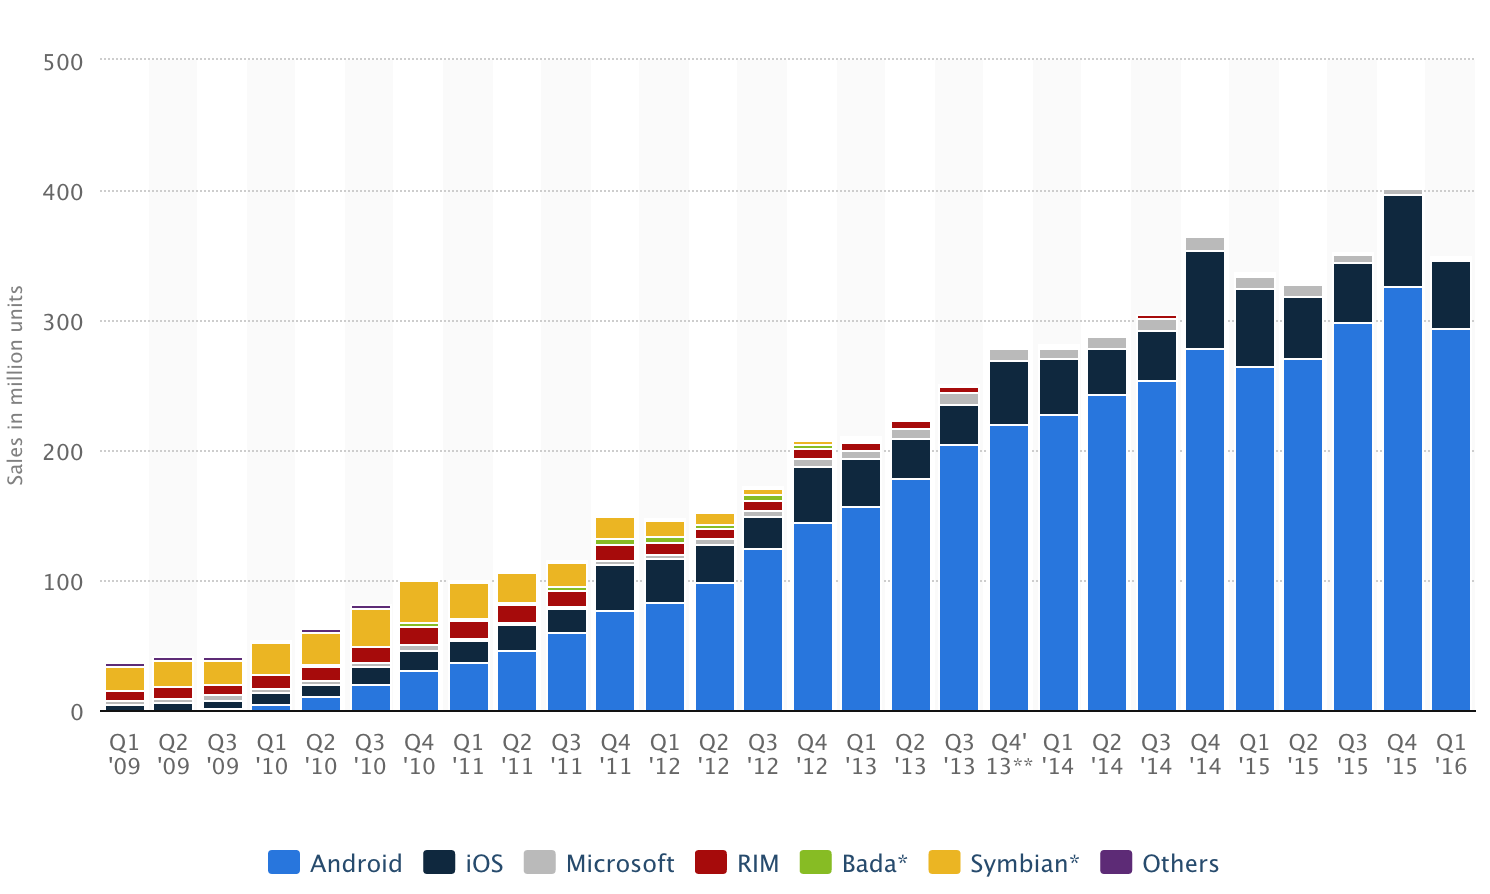
\includegraphics[width=0.9\textwidth]{mobile-market-share-bars.png}
	\caption{Unidades de dispositivos vendidos por plataforma m�vel \cite{SmartphoneSales:09-16}.}
	\label{fig:AndroidMarketShare}
\end{figure}

Com o crescimento da plataforma, a demanda por aplicativos tamb�m aumentou. Na Figura \ref{fig:GooglePlayStore} � poss�vel acompanhar o crescimento da quantidade de aplicativos dispon�veis na Google Play Store \footnote{Google Play Store (originalmente Android Market) � a loja oficial de aplicativos Android. Pode ser acessada pelo URL https://play.google.com/store \cite{WikiGooglePlay}.} ao longo de 2009 at� 2016, sendo que nesse �ltimo ano, superou 200 milh�es de aplicativos dispon�veis \cite{AppInPlayStore:09-16}.

\begin{figure}[!htb]
	\centering
	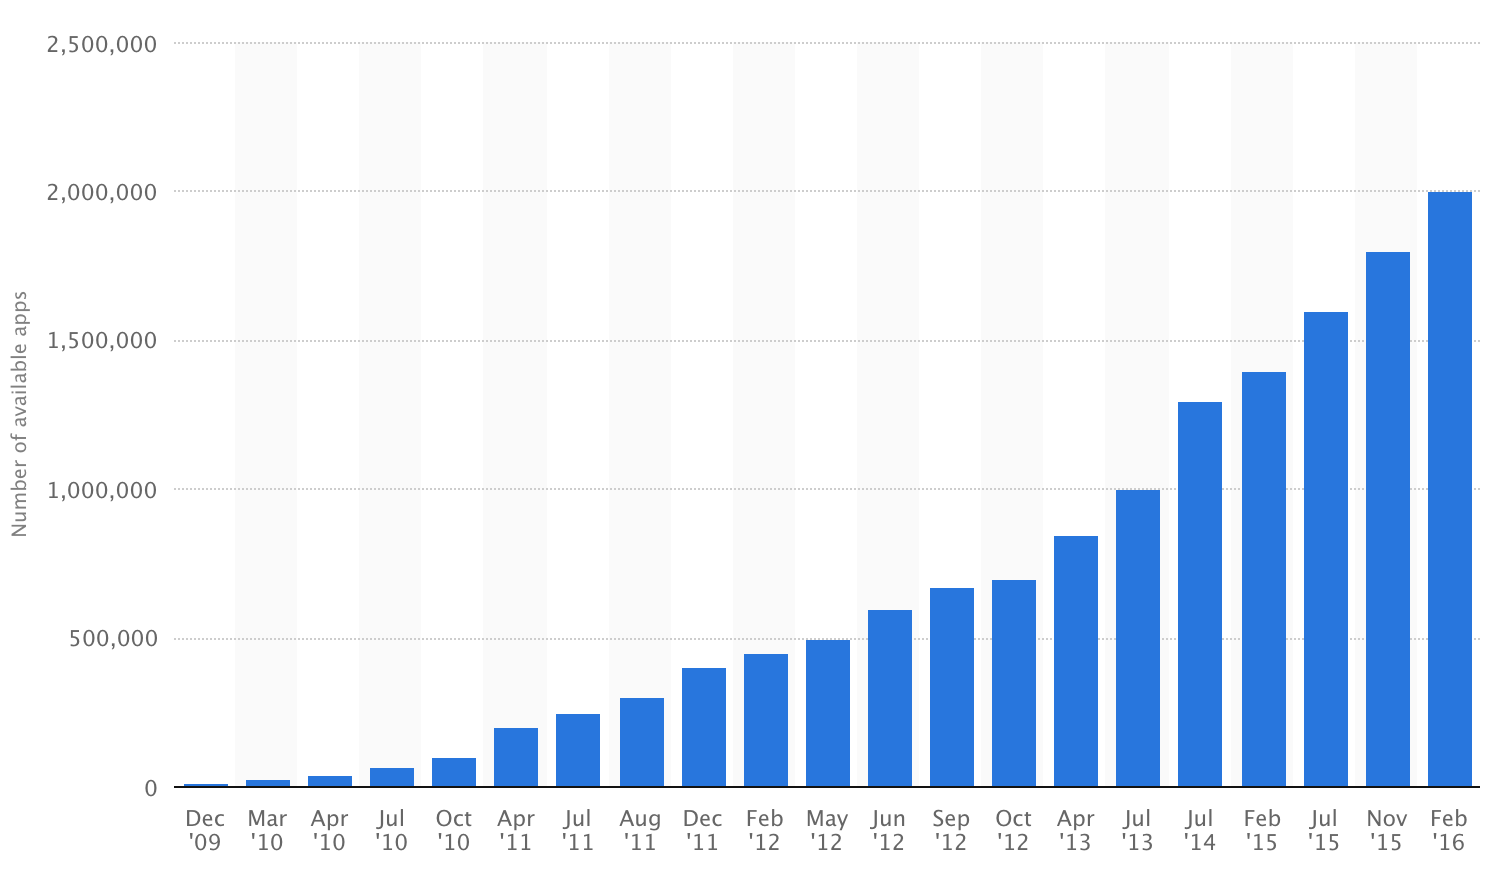
\includegraphics[width=0.9\textwidth]{play-store-apps-09to16.png}
	\caption{Quantidade de aplicativos dispon�veis na Google Play Store \cite{AppInPlayStore:09-16}.}
	\label{fig:GooglePlayStore}
\end{figure}


% \subsection{Arquitetura da Plataforma} 
Android � um sistema operacional de c�digo aberto, baseado no kernel do Linux criado para um amplo conjunto de dispositivos. Na Figura \ref{fig:AndroidPlatform} � apresentada a arquitetura geral da plataforma Android. Todas as funcionalidades da plataforma Android est�o dispon�veis para os aplicativos por meio de APIs Java (\textit{Application Programming Interface}). Essas APIs comp�em os elementos b�sicos para a constru��o de aplicativos Android.

% Para prover acesso aos recursos espec�ficos dos dispositivos como c�mera ou \textit{bluetooth}, o Android possui uma camada de abstra��o de \textit{hardware} (HAL do ingl�s \textit{Hardware Abstraction Layer}) exposto aos desenvolvedores por meio de um arcabou�o de Interfaces de Programa��o de Aplicativos Java (API - \textit{Applications Programming Interface}). 

% Estes e outros elementos explicados a seguir podem ser visualizados na Figura \ref{fig:AndroidPlatform} \cite{AndroidPlatformArchitecture}.

\begin{figure}[!htb]
	\centering
	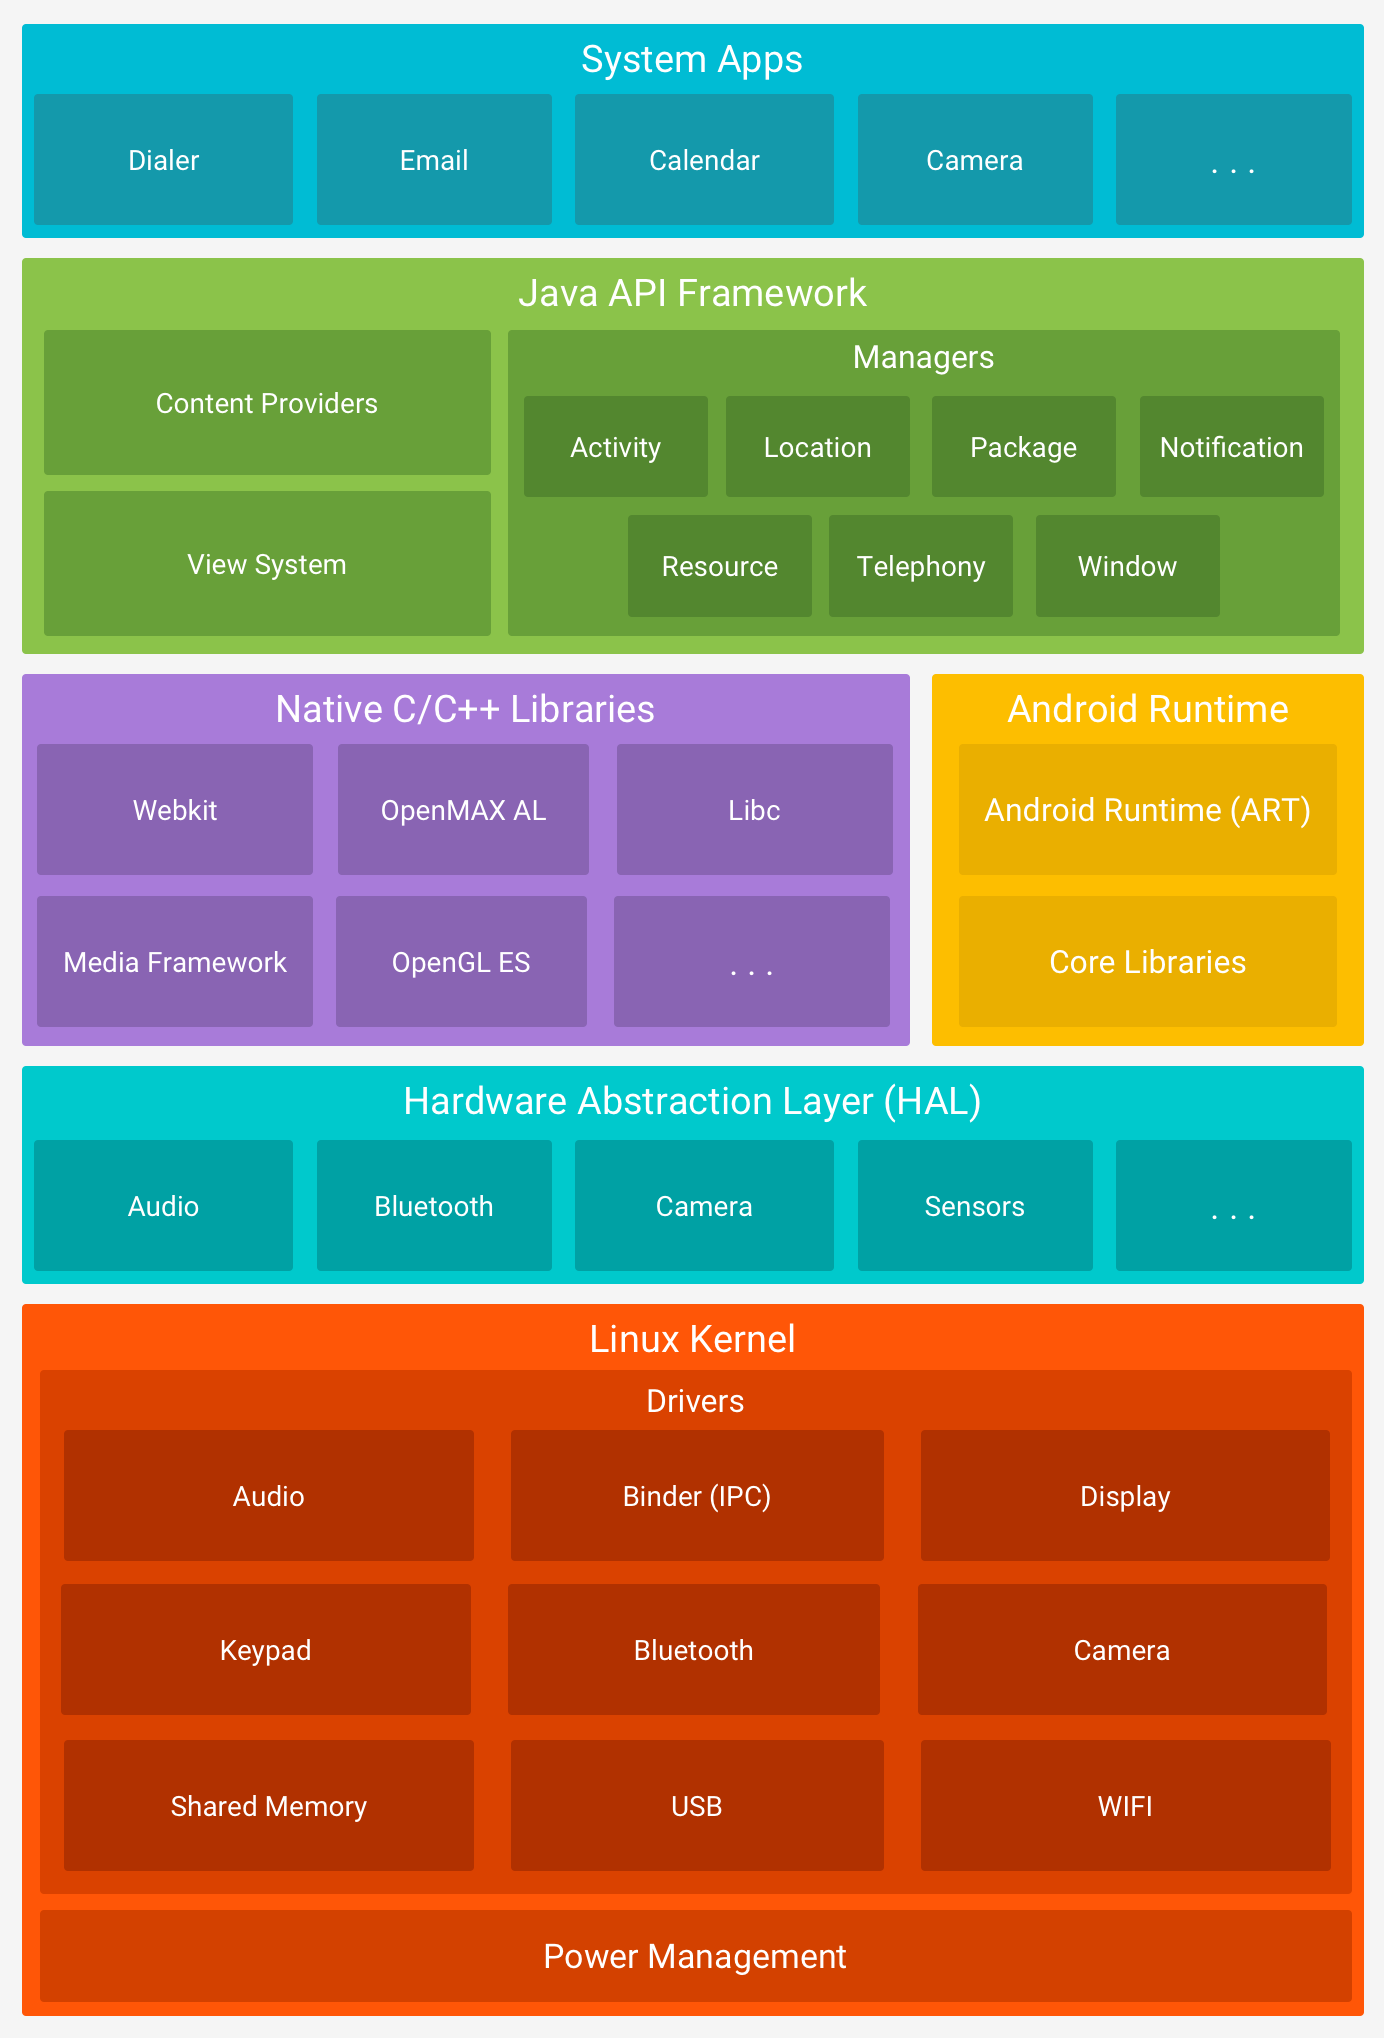
\includegraphics[width=0.7\textwidth]{android-architecture.png}
	\caption{Arquitetura do sistema operacional Android \cite{AndroidPlatformArchitecture}.}
	\label{fig:AndroidPlatform}
\end{figure}

% Cada aplicativo � executado em um novo processo de sistema que cont�m sua pr�pria inst�ncia do ambiente de execu��o Android. A partir da vers�o 5 (API n�vel 21), o ambiente de execu��o padr�o � o Android Runtime (ART), antes dessa vers�o era a Dalvik. ART foi escrita para executar multiplas inst�ncias de m�quina virtual em dispositivos com pouca mem�ria. Suas funcionalidades incluem: duas forma de compila��o, a frente do tempo (AOT do ingl�s \textit{Ahead-of-time}) e apenas no momento (JIT do ingl�s \textit{Just-in-time}), o coletor de lixo, ferramentas de depura��o e um relat�rio de diagn�sticos de erros e exce��es.

% Muitos dos componentes e servi�os b�sicos do Android, como ART e HAL, foram criados a partir de c�digo nativo que depende de bibliotecas nativas escritas em C e C++. A plataforma Android prov� arcabou�os de APIs Java para exp�r as funcionalidade de algumas dessas bibliotecas nativas para os aplicativos. Por exemplo, OpenGL ES pode ser acessado por meio do arcabou�o Android Java OpenGL API, de modo a adicionar suporte ao desenho e manipula��o de gr�ficos 2D e 3D no aplicativo.

% Todas as funcionalidades da plataforma Android est�o dispon�veis para os aplicativos por meio de APIs Java. Essas APIs comp�em os elementos b�sicos para a constru��o de aplicativos Android. 

% Dentre eles, os mais relevantes para esta disserta��o s�o:

% \begin{itemize}
% 	\item Um rico e extens�vel \textbf{Sistema de Visualiza��o} para a contru��o de interfaces com o usu�rio, tamb�m chamadas de arquivos de \textit{layout}, do aplicativo. Incluindo listas, grades ou tabelas, caixas de textos, bot�es, dentre outros.

% 	\item Um \textbf{Gerenciador de Recursos}, provendo acesso aos recursos ``n�o-java'' como textos, elementos gr�ficos, arquivos de \textit{layout}.

% 	\item Um \textbf{Gerenciador de Activity} que gerencia o ciclo de vida dos aplicativos e prov� uma navega��o comum.
% \end{itemize}

% O Android j� vem com um conjunto de aplicativos b�sicos como por exemplo, para envio e recebimento de SMS, calend�rio, navegador, contatos e outros. Esses aplicativos n�o possuem diferencial com rela��o aos aplicativos de terceiros. Todo aplicativo tem acesso ao mesmo arcabou�o de APIs do Android, seja ele aplicativo da plataforma ou de terceiro. Ou seja, um aplicativo de terceiro pode se tornar o aplicativo padr�o para navegar na internet, receber e enviar SMS e assim por diante.

% Aplicativos da plataforma prov�m capacidades b�sicas que aplicativos de terceiros podem reutilizar. Por exemplo, se um aplicativo de terceiro quer possibilitar o envio de SMS, o mesmo pode reutilizar o aplicativo de SMS existente, em vez de implementar tamb�m essa funcionalidade.

\subsection{Fundamentos do Desenvolvimento Android}

Aplicativos Android s�o escritos na linguagem de programa��o Java. O \ac{SDK} Android compila o c�digo, junto com qualquer arquivo de recurso ou dados, em um arquivo APK (\textit{Android Package}). Arquivos APKs, arquivo com extens�o \texttt{.apk}, s�o usados por dispositivos para a instala��o de aplicativos \cite{AndroidFundamentals}.

Os elementos base para a constru��o de aplicativos Android s�o os componentes. Cada componente � um diferente ponto de entrada por meio do qual o sistema aciona o aplicativo. Nem todos os componente s�o pontos de entrada para o usu�rio e alguns s�o dependentes entre si \cite{AndroidFundamentals}. H� quatro tipos diferentes de componentes Android, cada qual serve um prop�sito distinto e possui diferentes ciclos de vida, ou seja, como o componente � criado e destru�do \cite{AndroidFundamentals}. S�o eles:

\begin{itemize}

	\item \textbf{Activities}

	Uma \textit{activity} representa uma tela com uma interface de usu�rio. Por exemplo, um aplicativo de email pode ter uma \textit{activity} para mostrar a lista de emails, outra para redigir um email, outra para ler emails e assim por diante. Embora \textit{activities} trabalhem juntas de modo a criar uma experi�ncia de usu�rio (UX do ingl�s \textit{User Experience}) coesa no aplicativo de emails, cada uma � independente da outra. Desta forma, um aplicativo diferente poderia iniciar qualquer uma dessas \textit{activities} (se o aplicativo de emails permitir). Por exemplo, a \textit{activity} de redigir email no aplicativo de emails, poderia solicitar o aplicativo c�mera, de modo a permitir o compartilhamento de alguma foto. Uma \textit{activity} � implementada como uma subclasse de \texttt{Activity} \cite{AndroidFundamentals}.  

	\item \textbf{Services}

	Um \textit{service} � um componente que � executado em plano de fundo para processar opera��es de longa dura��o ou processar opera��es remotas. Um \textit{service} n�o prov� uma interface com o usu�rio. Por exemplo, um \textit{service} pode tocar uma m�sica em plano de fundo enquanto o usu�rio est� usando um aplicativo diferente, ou ele pode buscar dados em um servidor remoto atrav�s da internet sem bloquear as intera��es do usu�rio com a \textit{activity}. Um \textit{service} � implementado como uma subclasse de \texttt{Service} \cite{AndroidFundamentals}.

	\item \textbf{Content Providers}

	Um \textit{content provider} gerencia um conjunto compartilhado de dados do aplicativo. Estes dados podem estar armazenados em arquivos de sistema, banco de dados SQLite, servidor remoto ou qualquer outro local de armazenamento que o aplicativo possa acessar. Por meio de \textit{content providers}, outros aplicativos podem consultar ou modificar (se o \textit{content provider} permitir) os dados. Por exemplo, a plataforma Android disponibiliza um \textit{content provider} que gerencia as informa��es dos contatos dos usu�rios, possibilitando que qualquer aplicativo, com as devidas permiss�es, possa consultar, ler ou escrever informa��es sobre um contato. Um \textit{content provider} � implementado como uma subclasse de \texttt{ContentProvider} \cite{AndroidFundamentals}.

	\item \textbf{Broadcast Receivers}

	Um \textit{broadcast receiver} � um componente que responde a mensagens enviadas pelo sistema. Muitas destas mensagens s�o originadas da plataforma Android, por exemplo, o desligamento da tela, baixo n�vel de bateria e assim por diante. \textit{Broadcast receivers} n�o possuem interface de usu�rio. Para informar o usu�rio que algo ocorreu, \textit{broadcast receivers} podem criar notifica��es. Um \textit{broadcast receiver} � implementado como uma subclasse de \texttt{BroadcastReceiver} \cite{AndroidFundamentals}.

\end{itemize}

Para a plataforma iniciar quaisquer dos componentes mencionados, ela busca pela exist�ncia deles por meio da leitura do arquivo \texttt{AndroidManifest.xml} do aplicativo (arquivo de manifesto). O arquivo de manifesto � um arquivo XML, localizado na raiz do projeto, que cont�m informa��es sobre o aplicativo tais como: permiss�es de usu�rio, configura��es de depend�ncias do projeto, vers�o do Android, declara��es dos componentes do aplicativo, dentre outras \cite{AndroidFundamentals}. Por exemplo, uma \textit{activity} pode ser declarada conforme o C�digo-fonte \ref{lst:AndroidManifest}. \\

% Os elementos usados no arquivo de manifesto s�o definidos pelo vocabul�rio XML do Android. Por exemplo, uma \textit{activity} pode ser declarada conforme o C�digo-Fonte \ref{lst:AndroidManifest}. \\

\begin{lstlisting}[
	language=XML, 
	caption={Arquivo \texttt{AndroidManifest.xml}}, 
	label={lst:AndroidManifest}
]
<?xml version="1.0" encoding="utf-8"?>
<manifest ... >
    <application android:icon="@drawable/app_icon.png" ... >
        <activity android:name="com.example.project.ExampleActivity"
                  android:label="@string/example_label" ... >
        </activity>
        ...
    </application>
</manifest>	
\end{lstlisting}

No elemento \texttt{<application>}, o atributo \texttt{android:icon} aponta para o �cone, que � um recurso do tipo imagem, que identifica o aplicativo. No elemento \texttt{<activity>}, o atributo \texttt{android:name} especifica o nome completamente qualificado da \textit{Activity}, e por fim, o atributo \texttt{android:label} especifica um texto para ser usado como t�tulo da \textit{Activity}.

% Para declarar cada um dos quatro tipos de componentes, deve-se usar os elementos a seguir:
% \begin{itemize}
% 	\item \texttt{<activity>} elemento para \textit{activities}.
% 	\item \texttt{<service>} elemento para \textit{services}.
% 	\item \texttt{<receiver>} elemento para \textit{broadcast receivers}.
% 	\item \texttt{<provider>} elemento para \textit{content providers}.
% \end{itemize}

\subsection{Recursos do Aplicativo}
\label{sec:AndroidResources}

Um aplicativo Android � composto por outros arquivos al�m de c�digo Java, ele requer \textbf{recursos} como imagens, arquivos de �udio, anima��es, menus, estilos e qualquer recurso relativo a apresenta��o visual do aplicativo \cite{AndroidResourceType}. Recursos costumam ser arquivos XML que usam o vocabul�rio definido pelo Android \cite{AndroidFundamentals}.

Um dos aspectos mais importantes de prover recursos separados do c�digo-fonte � a habilidade de prover recursos alternativos para diferentes configura��es de dispositivos como por exemplo idioma ou tamanho de tela \cite{AndroidFundamentals}. Segundo levantamento, em 2015 foram encontrados mais de 24 mil dispositivos diferentes com Android \cite{AndroidFragmentation}.

Deve-se organizar os recursos dentro do diret�rio \texttt{res} do projeto, usando subdiret�rios que agrupam os recursos por tipo e configura��o. Para qualquer tipo de recurso, pode-se especificar uma op��o padr�o e outras alternativas \cite{AndroidFundamentals}. 

\begin{itemize}
	\item \textbf{Recursos padr�es} s�o aqueles que devem ser usados independente de qualquer configura��o ou quando n�o h� um recurso alternativo que atenda a configura��o atual. Por exemplo, arquivos de \textit{layout} padr�o ficam em \texttt{res/layout}.

	\item \textbf{Recursos alternativos} s�o todos aqueles que foram desenhados para atender a uma configura��o espec�fica. Para especificar que um grupo de recursos � para ser usado em determinada configura��o, basta adicionar um qualificador ao nome do diret�rio. Por exemplo, arquivos de \textit{layout} para quando o dispositivo est� em posi��o de paisagem ficam em \texttt{res/layout-land}.
\end{itemize}

O Android ir� aplicar automaticamente o recurso apropriado atrav�s da identifica��o da configura��o corrente do dispositivo. Por exemplo, o recurso do tipo \textit{strings} pode conter textos usados nas interfaces do aplicativo. � poss�vel traduzir estes textos em diferentes idiomas e salv�-los em arquivos separados. Desta forma, baseado no qualificador de idioma usado no nome do diret�rio deste tipo de recurso (por exemplo \texttt{res/values-fr} para o idioma franc�s) e a configura��o de idioma do dispositivo, o Android aplica o conjunto de \textit{strings} mais apropriado.

% A seguir s�o listados os tipos de recursos que podem ser utilizados no Android \cite{AndroidResourceType}. Para cada tipo de recurso existe um conjunto de qualificadores que podem ser usados para prover recursos alternativos:

% \begin{itemize}
% 	\item \textbf{Recursos de anima��es} Definem anima��es pr�-determinadas. Ficam nos diret�rios \texttt{res/anim} ou \texttt{res/animator}.

% 	\item \textbf{Recursos de lista de cores de estado} Definem recursos de cores que alteram baseado no estado da \textit{View}. Ficam no diret�rio \texttt{res/color}.	

% 	\item \textbf{Recursos de desenhos} Definem recursos gr�ficos como \textit{bitmap} ou XML. Ficam no diret�rio \texttt{res/drawable}.

% 	\item \textbf{Recursos de \textit{layouts}} Definem a parte visual da interface com o usu�rio. Ficam no diret�rio \texttt{res/layout}.

% 	\item \textbf{Recursos de menus} Definem os conte�dos dos menus da aplica��o. Ficam no diret�rio \texttt{res/menu}.

% 	\item \textbf{Recursos de textos} Definem textos, conjunto de textos e plurais. Ficam no diret�rio \texttt{res/values}.

% 	\item \textbf{Recursos de estilos} Definem os estilos e e formatos para os elementos da interface com usu�rio. Ficam no diret�rio \texttt{res/values}.

% 	\item \textbf{Outros recursos} Ainda existem outros recursos como inteiros, \textit{booleanos}, dimens�es, dentre outros. Ficam no diret�rio \texttt{res/values}.
% \end{itemize}


\subsection{Interfaces de Usu�rios}

\begin{figure}[!htb]
	\centering
	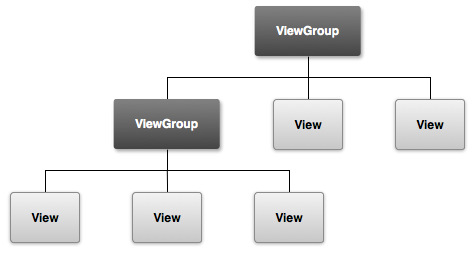
\includegraphics[width=0.7\textwidth]{ui-overview.png}
	\caption{�rvore hier�rquica de \texttt{View}s e \texttt{ViewGroup}s do Android \cite{AndroidUIOverview}.}
	\label{fig:UIOverview}
\end{figure}

Arquivos de \textit{layout} s�o recursos localizados no subdiret�rio \texttt{res/layout} que possuem a extens�o \texttt{.xml} \cite{AndroidResourceType}. Todos os elementos de UI (Interface de Usu�rio, do ingl�s UI, \textit{User Interface}) de um aplicativo Android s�o constru�dos usando objetos do tipo \texttt{View} e \texttt{ViewGroup} como mostrado na Figura \ref{fig:UIOverview} \cite{AndroidUIOverview}. 

Uma \texttt{View} � um objeto que desenha algo na tela do qual o usu�rio pode interagir como caixas de texto e bot�es. Um \texttt{ViewGroup} � um cont�iner invis�vel que organiza \texttt{View}s filhas. O encadeamento desses objetos formam uma �rvore hier�rquica que pode ser t�o simples ou complexa quanto se precisar \cite{AndroidResourceType}.

� poss�vel criar um \textit{layout} programaticamente instanciando \texttt{View}s e \texttt{ViewGroup}s no c�digo e construir a �rvore hier�rquica manualmente, no entanto, a forma mais indicada �  por meio de um XML de \textit{layout} \cite{AndroidUIOverview}. 

O vocabul�rio XML para declarar elementos de UI segue ou � muito pr�xima a estrutura de nome de classes e m�todos, onde os nomes dos elementos correspondem aos nomes das classes e os atributos correspondem aos nomes dos m�todos, como por exemplo, o elemento \texttt{<EditText>} tem o atributo \texttt{text} que corresponde ao m�todo \texttt{EditText.setText()} \cite{AndroidUIOverview}. Um layout vertical simples com uma caixa de texto e um bot�o se parece com o C�digo-fonte \ref{lst:LayoutSample}. \\

\begin{lstlisting}[
	language=XML, 
	caption={Arquivo exemplo de layout.}, 
	label={lst:LayoutSample}
]
<?xml version="1.0" encoding="utf-8"?>
<LinearLayout ...
              android:layout_width="fill_parent"
              android:layout_height="fill_parent"
              android:orientation="vertical">

    <TextView android:layout_width="wrap_content"
              android:layout_height="wrap_content"
              android:text="I am a TextView" />

    <Button   android:layout_width="wrap_content"
              android:layout_height="wrap_content"
              android:text="I am a Button" />

</LinearLayout>
\end{lstlisting}

% Quando um recurso de layout � carregado pelo aplicativo, o Android inicializa um objeto para cada elemento do layout, desta forma � poss�vel recuper�-lo programaticamente para definir comportamentos, modificar o layout ou mesmo recuperar o estado. 

% O Android prov� uma s�rie de elementos de UI comuns pr�-prontos como: caixa de texto, bot�o, lista suspensa, dentre muitos outros. Desta forma, o desenvolvedor n�o precisa implementar do zero estes elementos b�sicos atrav�s de \texttt{View}s e \texttt{ViewGroup}s para escrever uma interface de usu�rio.

% Cada subclasse de \texttt{ViewGroup} prov� uma forma �nica de exibir o conte�do dentro dele. Por exemplo, o \texttt{LinearLayout} organiza seu conte�do de forma linear horizontalmente, um ao lado do outro, ou verticalmente, um abaixo do outro. O \texttt{RelativeLayout} permite especificar a posi��o de uma \texttt{View} relativa ao posicionamento de alguma outra \cite{AndroidLayouts}.

Quando o conte�do � din�mico ou n�o pr�-determinado, como por exemplo uma lista de dados, pode-se usar um elemento que estende de \texttt{AdapterView} para popular o layout em tempo de execu��o. Subclasses de \texttt{AdapterView} usam uma implementa��o de \texttt{Adapter} para carregar dados em seu \textit{layout}. \texttt{Adapter}s agem como um intermediador entre o conte�do a ser exibido e o \textit{layout}, ele recupera o conte�do e converte cada item, de uma lista por exemplo, dentro de uma ou mais \texttt{View}s.

Os elementos comumente usados para situa��es de conte�do din�mico ou n�o pr�-determinado s�o: \texttt{ListView} e \texttt{GridView}. Para fazer o carregamento dos dados o Android prov� alguns \texttt{Adapter}s como por exemplo o \texttt{ArrayAdapter} que a partir de um \texttt{array} de dados popula os dados na \texttt{ListView} ou \texttt{GridView}.

Para responder a a��es do usu�rio, cada \texttt{View} possui um conjunto de interfaces que podem responder a eventos, essas interfaces s�o chamadas de \textit{event listeners}. Por exemplo, quando um bot�o � clicado, o evento \texttt{onClick} da interface \texttt{OnClickListener} � disparado. Ao associar a interface implementada ao bot�o, � poss�vel implementar a resposta desejada para essa a��o do usu�rio \cite{AndroidUIEvents}.

\subsection{Camada de Apresenta��o Android}
\label{ch:PresentationLayer}

Um assunto essencial para o entendimento deste trabalho � explanar o que queremos dizer com ``Camada de Apresenta��o Android''. Nesta se��o abordamos justamente este assunto com o objetivo de explanar como chegamos na defini��o aqui usada.

Em nossas pesquisas bibliogr�ficas n�o foi encontrada uma defini��o formal sobre camada de apresenta��o Android. Encontramos por�m, pontos na documenta��o oficial do Android \cite{AndroidDeveloperSite2016} que afirmam que determinado elemento de alguma forma � parte desta camada. Por exemplo o trecho sobre \textit{Activities} diz que ``representa uma tela com interface do usu�rio''. O trecho sobre recursos do aplicativo afirma que ``um aplicativo Android � composto por outros arquivos al�m de c�digo Java, ele requer recursos como imagens, arquivos de �udio e qualquer recurso relativo a apresenta��o visual do aplicativo'' \cite{AndroidFundamentals}. Encontramos tamb�m postagens em sites t�cnicos sobre Android que de alguma forma indicam que determinado elemento comp�e a camada de apresenta��o Android, por exemplo Preussler relaciona \textit{adapters} como parte da camada de apresenta��o \cite{AdaptersPreussler2016}. Desta forma viu-se necess�rio definir quais s�o os elementos, para efeitos desta disserta��o, que comp�em a camada de apresenta��o em aplicativos Android. 

Os prim�rdios de GUI (\textit{Graphical User Interfaces} ou Interfaces de Usu�rio Gr�ficas) foram em 1973 com o projeto Alto, desenvolvido pelos pesquisadores da Xerox Palo Alto Research Center (PARC), seguido do projeto Lisa da Apple em 1979. Estes dois projetos serviram de base e inspira��o para o Machintosh, lan�ado pela Apple em 1985. As primeiras defini��es sobre GUI que surgiram nessa �poca abordavam sobre componentes de uso comum como �cones, janelas, barras de rolagem, menus suspensos, bot�es, caixas de entrada de texto; gerenciadores de janelas; arquivos de �udio, internacionaliza��o e eventos. Antes deste per�odo existiam apenas interfaces de linha de comando \cite{GUIRaymond2004, UITecMundo2016}.

Outra fonte define camada de apresenta��o como ``informa��es gr�ficas, textuais e auditivas apresentadas ao utilizador, e as sequ�ncias de controle (como comandos de teclado, \textit{mouse} ou toque) para interagir com o programa'' \cite{UIWikipedia2016}. 

Unindo as defini��es supracitadas, definimos que todos os elementos do Android que s�o apresentados ou interagem com o usu�rio de alguma forma auditiva, visual ou por comando de voz ou toque s�o elementos da \textbf{Camada de Apresenta��o}, s�o eles:

\begin{itemize}
	\item \textbf{Activities e Fragments} Representam uma tela ou um fragmento de tela. A exemplo temos classes Java que herdam de \texttt{Activity}, \texttt{Fragment} ou classes similares.

	\item \textbf{Listeners} Meio pelo qual os comandos do usu�rio s�o capturados pelo aplicativo. A exemplo temos classes Java que implementam interfaces como \texttt{View.OnClickListener}.

	\item \textbf{Recursos do Aplicativo} Arquivos que apresentam textos, imagens, �udios, menus, interfaces gr�ficas (\textit{layout}), dentre outros. Est�o inclu�dos neste item todos os arquivos dentro do diret�rio \texttt{res} ainda que em seu formato Java. A exemplo podemos citar classes que herdam da classe \texttt{View} ou \texttt{ViewGroup}.

	\item \textbf{Adapters} Meio pelo qual s�o carregados conte�dos din�micos ou n�o pr�-determinados na tela. A exemplo podemos citar classes que herdam da classe \texttt{BaseAdapter}.

\end{itemize}

 
% -*- root: article.tex -*-
Muitas pesquisas t�m sido realizadas sobre a plataforma Android, muitas delas focam em vulnerabilidades \cite{Y, F, G, X, P, D, E}, autentica��o \cite{T, Yamashita6405287, R} e testes \cite{J, M}. Diferentemente dessas pesquisas, nossa pesquisa tem foco na percep��o dos desenvolvedores sobre boas e m�s pr�icas de desenvolvimento na plataforma Android. 

A percep��o desempenha um importante papel na defini��o de code smells relacionados a uma tecnologia, visto que code smells possuem uma natureza subjetiva. Code smells desempenham um importante papel na busca por qualidade de c�digo, visto que, ap�s mapeados, podemos chegar a heur�sticas para identific�-los e com essas heur�sticas, implementar ferramentas que automatizem o processo de identificar c�digos problem�ticos.

Verloop \cite{MobileSmells:13} conduziu um estudo no qual avaliou por meio de 4 ferramentas de detec��o automatizada de cheiros de c�digo (JDeodorant, Checkstyle, PMD e UCDetector) a presen�a de 5 cheiros de c�digo (Long Method, Large Class, Long Parameter List, Feature Envy e Dead Code) em 4 projetos Android. Nossa pesquisa se relaciona com a de Verloop no sentido de que tamb�m estamos buscando por cheiros de c�digo, entretanto, em vez de de buscarmos por cheiros de c�digo j� definidos, realizamos uma abordagem inversa na qual, primeiro buscamos entender a percep��o de desenvolvedores sobre boas e m�s pr�ticas em Android, e a partir dessa percep��o, relacionamos com algum cheiro de c�digo pr�-existente ou derivamos algum novo.

Gottschalk et al \cite{EnergyAndroidSmells} conduziram um estudo sobre formas de detectar e refatorar cheiros de c�digo relacionados ao uso efici�nte de energia. Os autores compilaram um cat�logo com 8 cheiros de c�digo e trabalharam sob um trecho de c�digo Android para exemplificar um deles, o "binding resource too early", quando algum recurso � alocado muito antes de precisar ser utilizado. Essaq pesquisa � relacionada \`a nossa por ambas considerarem a tecnologia Android e se diferenciam pois focamos na busca por cheiros de c�digo relacionados a qualidade de c�digo, no sentido de legibilidade e manutenablidade.

Aplicativos Android s�o escritos na linguagem de programa��o Java \cite{AndroidFundamentals}. Ent�o a primeira quest�o �: por que buscar por \textit{smells} Android sendo que j� existem tantos \textit{smells} Java? Pesquisas t�m demonstrado que tecnologias diferentes podem apresentar \textit{code smells} espec�ficos, como por exemplo Aniche et al. identificaram 6 \textit{code smells} espec�ficos ao framework Spring MVC, um framework Java para desenvolvimento web. Outras pesquisas concluem que projetos Android possuem caracter�sticas diferentes de projetos java \cite{Hecht2015, Mannan_Dig_Ahmed_Jensen_Abdullah_Almurshed, ReimannBrylski2013}, por exemplo, o \textit{front-end} � representado por arquivos XML e o ponto de entrada da aplica��o � dado por \textit{event-handler} \cite{AndroidActivities2016} como o m�todo \textsc{onCreate}. Encontramos tamb�m diversas pesquisas sobre \textit{code smells} sobre tecnologias usadas no desenvolvimento de \textit{front-end} web como CSS \cite{CSSCodeSmell} e JavaScript \cite{BB}. Essas pesquisas nos inspiraram a buscar entender se existem \textit{code smells} no \textit{front-end} Android. \\
% 
% Umme et al. \cite{Mannan_Dig_Ahmed_Jensen_Abdullah_Almurshed} recentemente levantaram que, das principais confer�ncias de manuten��o de software (ICSE, FSE, OOPSLA/SPLASH, ASE, ICSM/ICSME, MRS e ESEM), dentre 2008 a 2015, apenas 10\% dos artigos consideraram em suas pesquisas, projetos Android. Nenhuma outra plataforma m�vel foi considerada.  
% \textbf{[se��o n�o finalizada, � concluir.]}
% % -*- root: dissertacao.tex -*-
%%%%%%%%%%%%%%%%%%%%%%%%%%%%%%%%%%%%%%%%%%%%%%%%%%%%%%%%%%%%%%%%%%%%%%%
\setlength{\parindent}{20pt}
\setlength{\textheight}{22cm}
\setlength{\parskip}{0.2cm}
\linespread{1.2} % Para aumentar o espa�amento entre as linhas
%%%%%%%%%%%%%%%%%%%%%%%%%%%%%%%%%%%%%%%%%%%%%%%%%%%%%%%%%%%%%%%%%%%%%%%

\chapter{Camada de Apresenta��o Android}
\label{ch:PresentationLayer}

Um assunto essencial para o entendimento deste trabalho � explanar o que queremos dizer com ``Camada de Apresenta��o Android''. Nesta se��o abordamos justamente este assunto de forma a explanar como chegamos na defini��o aqui usada.

Em nossas pesquisas bibliogr�ficas n�o foi encontrada uma defini��o formal sobre camada de apresenta��o Android. Encontramos por�m, pontos na documenta��o oficial do Android \cite{AndroidDeveloperSite2016} que afirmam que determinado elemento de alguma forma � parte desta camada. Por exemplo o trecho sobre \textit{Activities} diz que ``representa uma tela com interface do usu�rio''. O trecho sobre recursos do aplicativo afirma que ``um aplicativo Android � composto por outros arquivos al�m de c�digo Java, ele requer recursos como imagens, arquivos de �udio e qualquer recurso relativo a apresenta��o visual do aplicativo'' \cite{AndroidFundamentals}. Encontramos tamb�m postagens em sites t�cnicos sobre Android que de alguma forma indicam que determinado elemento comp�e a camada de apresenta��o Android, por exemplo Preussler relaciona \textit{adapters} como parte da camada de apresenta��o \cite{AdaptersPreussler2016}. Desta forma viu-se necess�rio definir quais s�o os elementos, para efeitos desta disserta��o, que comp�em a camada de apresenta��o em aplicativos Android. 

Os prim�rdios de GUI (\textit{Graphical User Interfaces} ou Interfaces de Usu�rio Gr�ficas) foram em 1973 com o projeto Alto, desenvolvido pelos pesquisadores da Xerox Palo Alto Research Center (PARC), seguido do projeto Lisa da Apple em 1979. Estes dois projetos serviram de base e inspira��o para o Machintosh, lan�ado pela Apple em 1985. As primeiras defini��es sobre GUI que surgiram nessa �poca abordavam sobre componentes de uso comum como �cones, janelas, barras de rolagem, menus suspensos, bot�es, caixas de entrada de texto; gerenciadores de janelas; arquivos de �udio, internacionaliza��o e eventos. Antes deste per�odo existiam apenas interfaces de linha de comando \cite{GUIRaymond2004, UITecMundo2016}.

Outra fonte define camada de apresenta��o como ``informa��es gr�ficas, textuais e auditivas apresentadas ao utilizador, e as sequ�ncias de controle (como comandos de teclado, \textit{mouse} ou toque) para interagir com o programa'' \cite{UIWikipedia2016}. 

Unindo as defini��es supracitadas, definimos que todos os elementos do Android que s�o apresentados ou interagem com o usu�rio de alguma forma auditiva, visual ou por comando de voz ou toque s�o elementos da \textbf{Camada de Apresenta��o}, s�o eles:

\begin{itemize}
	\item \textbf{Activities e Fragments} Representam uma tela ou um fragmento de tela. A exemplo temos classes Java que herdam de \texttt{Activity}, \texttt{Fragment} ou classes similares.

	\item \textbf{Listeners} Meio pelo qual os comandos do usu�rio s�o capturados pelo aplicativo. A exemplo temos classes Java que implementam interfaces como \texttt{View.OnClickListener}.

	\item \textbf{Recursos do Aplicativo} Arquivos que apresentam textos, imagens, �udios, menus, interfaces gr�ficas (\textit{layout}), dentre outros. Est�o inclu�dos neste item todos os arquivos dentro do diret�rio \texttt{res} ainda que em seu formato Java. A exemplo podemos citar classes que herdam da classe \texttt{View} ou \texttt{ViewGroup}.

	\item \textbf{Adapters} Meio pelo qual s�o carregados conte�dos din�micos ou n�o pr�-determinados na tela. A exemplo podemos citar classes que herdam da classe \texttt{BaseAdapter}.

\end{itemize}


% -*- root: dissertacao.tex -*-
%%%%%%%%%%%%%%%%%%%%%%%%%%%%%%%%%%%%%%%%%%%%%%%%%%%%%%%%%%%%%%%%%%%%%%%
\setlength{\parindent}{20pt}
\setlength{\textheight}{22cm}
\setlength{\parskip}{0.2cm}
\linespread{1.2} % Para aumentar o espa�amento entre as linhas
%%%%%%%%%%%%%%%%%%%%%%%%%%%%%%%%%%%%%%%%%%%%%%%%%%%%%%%%%%%%%%%%%%%%%%%

\chapter{Proposta de Disserta��o}

Conforme apresentado no Cap�tulo 1, podem existir maus cheiros espec�ficos a um dom�nio, tecnologia ou plataforma (por exemplo, Android) \cite{FinavaroAniche2016, DomainMatters, MobileSmells:13}. Geoffrey \cite{Hecht2015} afirma que a detec��o e especifica��o de padr�es m�veis ainda � um problema em aberto e que \textit{antipatterns} Android s�o mais frequentes em projetos m�veis do que \textit{antipatterns} orientado a objetos. Pesquisas em torno de projetos de aplicativos m�veis ainda s�o poucas \cite{Mannan_Dig_Ahmed_Jensen_Abdullah_Almurshed}. Desta forma, neste cap�tulo � apresentada a proposta da disserta��o e o cronograma de atividades planejadas. 


\section{Atividades}

Para obter as ideias iniciais para a deriva��o dos maus cheiros na camada de apresenta��o Android, foi aplicado um question�rio sobre boas e m�s pr�ticas Android na comunidade de desenvolvedores do Brasil e exterior. O question�rio pode ser encontrado no Ap�ndice A e at� o momento da escrita desta proposta de qualifica��o foram coletadas 44 respostas. Ainda de modo a complementar os dados coletados com o question�rio, pretende-se realizar entrevista com desenvolvedores Android sobre o mesmo tema. Tamb�m ser� feito uma an�lise para derivar os maus cheiros, essa an�lise ser� feita com base em estrat�gias j� utilizadas em trabalhos anteriores como o de Aniche et al. \cite{FinavaroAniche2016}. Para reduzir vi�s sobre os maus cheiros definidos, os mesmos ser�o validados com mais de um especialista em Android. A deriva��o dos maus cheiros est� relacionada a Q1 definida na se��o 1.1 e as atividades planejadas s�o:

\begin{itemize} 
	\item Bibliografia e Trabalhos Relacionados.
	\item Survey Boas e M�s pr�ticas Android.
	\item Deriva��o dos Maus Cheiros.
	\item Valida��o Maus Cheiros c/ Especialista.
\end{itemize}

Evid�ncias na literatura sugerem que maus cheiros de c�digo podem esconder manutenibilidade de c�digo \cite{Sjoberg_Quantifying_2013, Yamashita6405287, Yamashita:2013:EII:2486788.2486878} e aumentar a tend�ncia a mudan�as e introdu��o de defeitos \cite{Khomh:2009:ESI:1685994.1686210, Khomh:2012:ESI:2158916.2158921}. Mario et al. \cite{DomainMatters} mostra que \textit{antipatterns} impactam negativamente m�tricas relacionadas a qualidade em projetos m�veis, em particular m�tricas relacionadas a propens�o de falhas. Desta forma, pretende-se avaliar o impacto dos maus cheiros propostos na tend�ncia a mudan�as e introdu��o de defeitos no c�digo. Para isso ser� realizado um experimento presencial com desenvolvedores Android. Este experimento est� relacionado ao Q2 definida na Se��o 1.1 e a atividade planejada �:

\begin{itemize} 
	\item Experimento Impacto em Mudan�as/Defeitos.
\end{itemize}

Evid�ncias na literatura tamb�m sugerem que maus cheiros de c�digo s�o percebidos por desenvolvedores \cite{Palomba_Do_2014}, desta forma pretende-se avaliar se desenvolvedores Android percebem c�digos afetados pelos maus cheiros propostos como indicativos de trechos de c�digos ruins. Para isso ser� conduzido outro experimento tamb�m com desenvolvedores Android. Esse experimento est� relacionado a Q3 definida na Se��o 1.1 e a seguinte atividade est� planejada:

\begin{itemize} 
	\item Experimento Percep��o Desenvolvedores.
\end{itemize}


\section{Cronograma}

Na Tabela \ref{tab:Cronograma} s�o apresentadas as atividades previstas para a conclus�o da disserta��o bem como em qual per�odo pretende-se realiz�-la.

\begin{table}[h]
\centering

\newcommand\T{\rule{0pt}{2.6ex}}       % Top strut
\newcommand\B{\rule[-1.2ex]{0pt}{0pt}} % Bottom strut

\begin{tabular}{|l|cc|cccc|} 
\hline
\multicolumn{1}{|c|}{} 	& \multicolumn{2}{c|}{2016}   	& \multicolumn{4}{c|}{2017} \\
\textbf{Atividades}		& 3$^o$ Tri & 4$^o$ Tri 		& 1$^o$ Tri & 2$^o$ Tri & 3$^o$ Tri & 4$^o$ Tri \\
\hline
\hline
% \rule{0pt}{-1em} 		& 			& 					& 			& 			&			&			\\
Bibliografia e Trabalhos Relacionados 	& \textbullet 	& \textbullet	& 				& 				& 				& 				\T \\
Survey Boas e M�s pr�ticas Android 		& 				& \textbullet	& 				& 				& 				& 				\\
Entrevista Boas e M�s pr�ticas Android	& 				& 				& \textbullet	& 				& 				& 				\\
Deriva��o dos Maus Cheiros 				& 				& 				& \textbullet	& 				& 				& 				\\
Valida��o Maus Cheiros c/ Especialista	& 				& 				& \textbullet	& 				& 				& 				\\
Experimento Impacto em Mudan�as/Defeitos	& 				& 				& 				& \textbullet	& 				& 				\\
Experimento Percep��o Desenvolvedores	& 				& 				& 				& \textbullet 	& 				& 				\\
Escrita da Disserta��o					& \textbullet	& \textbullet	& \textbullet	& \textbullet	& \textbullet	& \textbullet	\\
Defesa									& 				& 				& 				& 				& 				& \textbullet	\B \\
\hline
\end{tabular}
\caption{Cronograma de atividades propostas.}
\label{tab:Cronograma}
\end{table} 
% \include{research} 
% % -*- root: article.tex -*-
% Neste artigo investigamos a exist�ncia de boas e m�s pr�ticas no \textit{front-end} de projetos Android. Fizemos isso atrav�s de um estudo explorat�rio qualitativo com 45 desenvolvedores, onde mapeamos 23 m�s pr�ticas Android. Ap�s, validamos a percep��o de desenvolvedores Android sobre as quatro m�s pr�ticas mais recorr�ntes. Fizemos isso atrav�s de um experimento online respondido com 20 desenvolvedores Android. Respondemos a \textbf{QP1} com um cat�logo com 23 m�s pr�ticas no \textit{front-end} Android. Respondemos a \textbf{QP2} atrav�s da valida��o com sucesso da percep��o de desenvolvedores sobre 2 das m�s pr�ticas de alta recorr�ncia.

% Neste artigo investigamos a exist�ncia de boas e m�s pr�ticas no \textit{front-end} de projetos Android. Fizemos isso atrav�s de um estudo explorat�rio qualitativo com 45 desenvolvedores, onde mapeamos 23 m�s pr�ticas Android. Ap�s, validamos a percep��o de desenvolvedores Android sobre as quatro m�s pr�ticas mais recorr�ntes. Fizemos isso atrav�s de um experimento online respondido com 20 desenvolvedores Android. 

% Respondemos a \textbf{QP1} com um cat�logo com 23 m�s pr�ticas no \textit{front-end} Android. Respondemos a \textbf{QP2} atrav�s da valida��o com sucesso da percep��o de desenvolvedores sobre 2 das m�s pr�ticas de alta recorr�ncia.

Neste artigo investigamos a exist�ncia de boas e m�s pr�ticas em elementos usados para implementa��o de \textit{front-end} de projetos Android: \textsc{Activities}, \textsc{Fragments}, \textsc{Listeners}, \textsc{Adapters}, \textsc{Layout}, \textsc{Styles}, \textsc{String} e \textsc{Drawable}. Fizemos isso atrav�s de um estudo explorat�rio qualitativo onde coletamos dados por meio de um question�rio online respondido por 45 desenvolvedores Android. A partir deste question�rio mapeamos 23 m�s pr�ticas e sugest�es de solu��o, quando mencionado por algum participante. Ap�s, validamos a percep��o de desenvolvedores Android sobre as quatro mais recorr�ntes dessas m�s pr�ticas: \textsc{L�gica em Classes de UI}, \textsc{Nome de Recurso Despadronizado}, \textsc{Recurso M�gico e Layout Profundamente Aninhado}. Fizemos isso atrav�s de um experimento online respondido por 20 desenvolvedores Android, onde os participantes eram convidados a avaliar 6 c�digos com rela��o a qualidade. \\

\textbf{QP1.} \textbf{O que desenvolvedores consideram boas e m�s pr�ticas no desenvolvimento Android?} 

Questionamos 45 desenvolvedores sobre o que eles consideravam boas e m�s pr�ticas em elementos espec�ficos do Android. Com base nesses dados, consolidamos um cat�logo com 23 m�s pr�ticas onde, para cada uma delas apresentamos uma descri��o textual e exemplos de frases usadas nas respostas que nos levaram a sua defini��o. \\

\textbf{QP2.} \textbf{C�digos afetados por estas m�s pr�ticas s�o percebidos pelos desenvolvedores como problem�ticos?}

Validamos a percep��o de desenvolvedores sobre as quatro m�s pr�tica mais recorr�ntes. Conclu�mos que desenvolvedores de fato as percebem como m�s pr�ticas. Duas das m�s pr�ticas, \textsc{L�gica em Classes de UI} e \textsc{Layout Profundamente Aninhado} foram poss�veis confirmar com dados estat�sticos. Outras duas, \textsc{Nome de Recurso Despadronizado} e \textsc{Recurso M�gico}, embora os dados estat�sticos n�o tenham confirmado, notamos por meio das respostas abertas que existe esta percep��o.



 


\appendix

%%%%%%%%%%%%%%%%%%%%%%%%%%%%%%%%%%%%%%%%%%%%%%%%%%%%%%%%%%%%%%%%%%%%%%%
\setlength{\parindent}{0pt}
\setlength{\textheight}{22cm}
\setlength{\parskip}{0.2cm}

% Para aumentar o espa�amento entre as linhas
\linespread{1.2}
%%%%%%%%%%%%%%%%%%%%%%%%%%%%%%%%%%%%%%%%%%%%%%%%%%%%%%%%%%%%%%%%%%%%%%%

\chapter{XYZ}

\section{Ap�ndice 1}

A fazer. \\


%%%%%%%%%%%%%%%%%%%%%%%%%%%%%%%%%%%%%%%%%%%%%%%%%%%%%%%%%%%%%%%%%%%%%%%%%

\onehalfspacing
\bibliographystyle{plain}
\bibliography{bibliografias}

\printindex

\end{document}
